\section{Вероятностные меры на $(\mathbb{R}^n,\, \mathcal{B}(\mathbb{R}^n))$}
\begin{definition}
	Функцией распределения вероятностной меры $P$ называется $F(x_1,\,\cdots,\,x_n),\, x_i \in \mathbb{R},\, i = \overline{1,\,n}$, где
	\[F(x_1,\,\cdots,\,x_n) = P((-\infty,\,x_1]\times\cdots\times (-\infty,\, x_n])\]
\end{definition}

\begin{note}
	\begin{enumerate}
		\item $\vec{x} = (x_1,\,\cdots,\,x_n)$
		\item $\vec{x} \geq \vec{y}$, если
		      \[\forall i = \overline{1,\,n}:\: x_i \geq y_i\]
		\item $(-\infty,\,\vec{x}] = (-\infty,\,x_1]\times\cdots\times (-\infty,\, x_n]$
		\item $\vec{x}_{(n)} \downarrow \vec{x}$, если
		      \[\forall n \in \mathbb{N}:\: \vec{x}_{(n)} \geq \vec{x}_{(n + 1)} \geq \vec{x}\]
		      причём $\lim_n \vec{x}_{(n)} = \vec{x}$
	\end{enumerate}
\end{note}

\begin{lemma}
	Свойства многомерной функции распределения.

	Пусть $F(\vec{x})$ -- функция распределения вероятностной меры $P$ на $(\mathbb{R}^n,\, \mathcal{B}(\mathbb{R}^n))$. Тогда
	\begin{enumerate}
		\item Если $\vec{x}_{(n)} \downarrow \vec{x}$, то
		      \[\lim_{n \to +\infty} F(\vec{x}_{(n)}) = F(\vec{x})\]
		      то есть непрерывна справа по любой координате
		\item Если $x_i \to +\infty,\, \forall i = \overline{1,\,n}$, то
		      \[F(\vec{x}) \to 1\]
		      Если $x_i \to -\infty,\, \exists i = \overline{1,\,n}$, то
		      \[F(\vec{x}) \to 0\]
		\item Для $\forall i = \overline{1,\,n}$ и $a_i < b_i$ введём оператор $\bigtriangleup_{a_i,\,b_i}^i$, который действует следующим образом:
		      \[
			      \bigtriangleup_{a_i,\,b_i}^i F(\vec{x}) = F(x_1,\,\cdots,\,b_i,\,x_{i + 1},\,\cdots,\,x_n) - F(x_1,\,\cdots,\,a_i,\,x_{i + 1},\,\cdots,\,x_n)
		      \]
		      Тогда
		      \[\forall a_1 < b_1,\,\cdots,\, a_n < b_n:\: \bigtriangleup_{a_1,\,b_1}^1 \circ \cdots \circ \bigtriangleup_{a_n,\,b_n}^n F(\vec{x}) \geq 0\]
	\end{enumerate}
\end{lemma}

\begin{proof}
	\begin{enumerate}
		\item Если $\vec{x}_{(n)} \downarrow \vec{x}$, то $(-\infty,\, \vec{x}_{(n)}] \downarrow (-\infty,\, \vec{x}]$. Тогда по непрерывности меры
		      \[
			      F(\vec{x}_{(n)}) = P((-\infty,\, \vec{x}_{(n)}]) \stackrel{n \to +\infty}{\to} P((-\infty,\, \vec{x}]) = F(\vec{x})
		      \]
		\item Если $\vec{x} \uparrow (+\infty,\,\cdots,\,+\infty)$, то $(-\infty,\, \vec{x}] \uparrow \mathbb{R}^n$. Тогда по непрерывности меры
		      \[F(\vec{x}_{(n)}) = P((-\infty,\, \vec{x}_{(n)}]) \stackrel{n \to +\infty}{\to} P(\mathbb{R}^n) = 1\]
		      Если $x_i \downarrow -\infty$, то $(-\infty,\, \vec{x}] \downarrow \emptyset$. Тогда в силу непрерывности меры
		      \[F(\vec{x}_{(n)}) = P((-\infty,\, \vec{x}_{(n)}]) \stackrel{n \to +\infty}{\to} P(\emptyset) = 0\]
		\item Проверим, например для $n = 2$, что
		      \[\bigtriangleup_{a_1,\,b_1}^1 \circ \cdots \circ \bigtriangleup_{a_n,\,b_n}^n F(\vec{x}) = P((a_1,\,b_1] \times\cdots\times (a_n,\,b_n])\]
		      Действительно:
		      \begin{align*}
			      \bigtriangleup^1_{a_1,\,b_1} \circ\bigtriangleup^2_{a_2,\,b_2} F(x_1,\,x_2) = \bigtriangleup^1_{a_1,\,b_1} (F(x_1,\,b_2) - F(x_1,\,a_2)) = \\
			      F(b_1,\,b_2) - F(b_1,\,a_2) - F(a_1,\,b_2) + F(a_1,\,a_2) = P((a_1,\,b_1] \times (a_2,\,b_2]) \geq 0
		      \end{align*}
		      \begin{figure}[h]
			      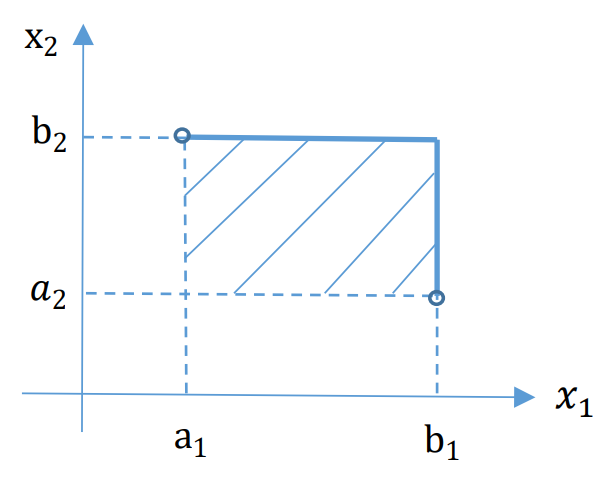
\includegraphics[scale=0.3]{img/f_example.png}
		      \end{figure}


		      В общем случае достаточно заметить, что
		      \[\bigtriangleup^i_{a_i,\,b_i}P(B_1\times\cdots\times B_{i - 1} \times (-\infty,\, x_i]\times\cdots\times B_n) = P(B_1\times\cdots\times(a_i,\,b_i]\times\cdots\times B_n)\]
	\end{enumerate}
\end{proof}

\begin{theorem}
	О построении вероятностной меры на $(\mathbb{R}^n,\, \mathcal{B}(\mathbb{R}^n))$ по функции распределения (б/д).

	Пусть $F(\vec{x})$ удовлетворяет всем свойствам из предыдущей леммы. Тогда $\exists!$ вероятностная мера на $(\mathbb{R}^n,\, \mathcal{B}(\mathbb{R}^n))$, для которой $F$ является функцией распределения.
\end{theorem}

\begin{definition}
	Пусть $P$ -- вероятностная мера на $(\mathbb{R}^\infty,\, \mathcal{B}(\mathbb{R}^\infty))$.

	$\forall n \in \mathbb{N}$ рассмотрим
	\[P_n(B) = P(F_n(B))\]
	где $F_n(B) = \{\vec{x} = (x_1,\,x_2,\,\cdots) :\: (x_1\,\,\cdots,\,x_n) \in B\}$ -- циллиндр с основанием $B$.

	Тогда $P_n$ будет вероятностной мерой в $\mathbb{R}^n$. Кроме того, $\forall n :\: \forall B \in \mathcal{B}(\mathbb{R}^n)$:
	\[P_n(B) = P_{n + 1}(B \times \mathbb{R})\]
	Это свойство согласованности.
\end{definition}

\begin{theorem}
	Колмогорова о мерах в $\mathbb{R}^\infty$ (б/д).

	Пусть $P_1,\,P_2,\,\cdots$ -- последовательность вероятностных мер в $\mathbb{R},\,\mathbb{R}^2,\,\cdots$, обладающая свойством согласованности.
	Тогда $\exists!$ вероятностная мера $P$ на $(\mathbb{R}^\infty,\,\mathcal{B}(\mathbb{R}^\infty))$, такая что
	\[\forall n \in \mathbb{N} \: \forall B \in \mathcal{B}(\mathbb{R}^n):\: P_n(B) = P(F_n(B))\]
\end{theorem}
